%----------------------------------------------------------------------------------------
\chapter{Related Work} % or Background
\label{chap:background}
%----------------------------------------------------------------------------------------

% intro 
In this chapter, we will proceed with the literature analysis and state-of-the-art methods related to the topic. Furthermore, some basic notions regarding the previous research relied upon will be explained.

Trajectory generation for robotics is a topic closely related to manipulation and navigation. Every movement can be described as a trajectory, defined as the composition of the path taken by an agent (or its joints) in time \cite{biagiotti2008trajectory}. 
In this discussion, we will focus more on the manipulation part, being the most clear example of how combining different trajectories can produce novel robotic skills. Manipulation is one of the most distinctive capabilities of robots, since their main objective is to perform physical tasks in the real world. Any process that presents the necessity of a human to engage with a physical object meaningfully can solely be automated by robot manipulation. \cite{rosen2022role}

Creating robots capable of directly interacting with the world around them is still a key challenge in robotics, and manipulation is central to this. \cite{kroemer2021review} 
Nevertheless, the ability to solve high-level goals in robots is increasing \cite{gupta2019relay}, \cite{simeonov2021long} thanks to the recent advances in artificial intelligence.  
Some approaches may follow natural language instructions to achieve complex sequences of actions \cite{hu2019hierarchical}, but according to the research objective, a certain degree of autonomy is desired. This implies typically giving only the final goal and not the step-by-step instructions. 

% some proposals
% Initial approaches utilized ... TODO
% latest proposals


% importance of Learning by Demonstration
A commonly used technique in robotics is Learning from Demonstration (LfD) \cite{ARGALL2009469}, and then \cite{ravichandar2020recent}. It allows for solving a wide variety of robotics problems by imitating an external agent. The demonstrator, often a human or another system, provides examples (expert demonstrations) of how to perform a task, and the learning agent generalizes from these demonstrations to acquire the ability to perform the task later independently.

Famous learning from demonstration research includes statistical modeling \cite{calinon2016tutorial}, dynamic systems \cite{schaal2006dynamic}, and their union in \cite{ugur2020compliant}. In Dynamic Movement Primitives (DMPs) \cite{schaal2006dynamic}, a trajectory is represented with a set of differential equations and learned with as little as one shot. Thanks to the "point attractor" mechanism, it guarantees reaching a point even under perturbations. DMPs have successfully been utilized in difficult manipulation tasks such as in-hand manipulation and flipping boxes using chopsticks \cite{pastor2009learning}. On the other hand, DMPs require additional tuning to determine the number of basis functions. Moreover, their approach is not designed to learn from multiple trajectories and, therefore, cannot encode the important parts of multiple demonstrations \cite{Ugur-RSS-19}. 

In the Probabilistic Movement Primitives (ProMP) \cite{paraschos2013probabilistic}, instead, the distribution of basis functions is often represented using a probabilistic framework, typically a Gaussian Mixture Model (GMM) or a similar probabilistic model. Historically, Gaussian Mixture Models \cite{nguyen2009model} have been prominent among various probabilistic approaches since they provide adaptable solutions to the challenge of modeling trajectories. On the other hand, GMMs involve estimating many parameters, especially when dealing with high-dimensional data or a large number of components. This can make training and inference computationally expensive, particularly when the dataset is extensive, and if not done correctly, can lead to some failures, Figure \ref{fig:prompcnmp}.
\begin{figure}
	\centering
	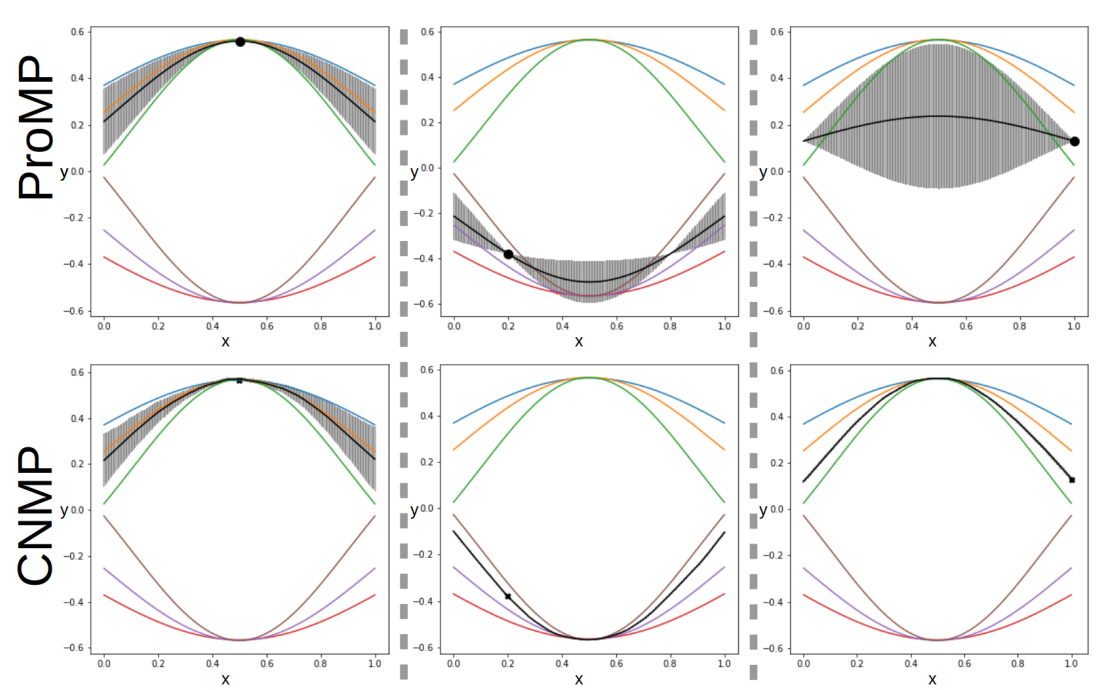
\includegraphics[width=0.5\linewidth]{Images/ProMPvsCNMP.png}
	\caption{In ProMPs the distribution of basis functions is often represented using a probabilistic framework, but can lead to some failures.}
	\label{fig:prompcnmp}
\end{figure}

Another probabilistic model, like GMMs, often used in statistical modeling techniques is Hidden Markov Models (HMMs) \cite{lee2011incremental}. HMMs were successfully applied to learn multi-modal models from temperature, pressure, and fingertip information for exploratory object classification tasks \cite{chu2013using}.

A recent model developed in robotics called Conditional Neural Movement Primitives (CNMP) \cite{Ugur-RSS-19} also learns from demonstrations, but instead of using GMMs, they use neural networks to model the mapping from conditions to trajectories directly. Neural networks allow the model to scale better and to offer robust data approximation via gradient descent. Until recently, neural networks in deep learning were trained to approximate a single-output function. However, when data is a distribution, the single function cannot approximate the underlying model. So the network can be modeled as a probabilistic approximator, that can predict the distribution parameters, mean, and variance. This makes CNMPs well-suited for tasks with complex, high-dimensional state spaces. It allows one to learn skills in tens, rather than thousands, of real-world interactions and interpolate among them.

% our proposal/contribution
Based on the above-mentioned observations, the proposal is as follows.
In the following research, the ability of CNMPs to interpolate the trajectories demonstrated is exploited to synthesize new complex skills. 
The model is based on Gaussian Processes (GP) \cite{seeger2004gaussian}, Neural Processes (NPs) \cite{garnelo2018neural}, and  Conditional Neural Processes (CNPs) \cite{DBLP:journals/corr/abs-1807-01613}.
For context, an explanation in detail of these above-mentioned methods will follow.



%%%%%%% BACKGROUND IN DEPTH %%%%%%%
%%%%%%% GP %%%%%%%
\section{Gaussian Processes}
Gaussian Processes \cite{seeger2004gaussian} are probabilistic models that define a distribution over functions, Figure \ref{fig:gp}.
This means that they leverage pre-existing knowledge about a set of functions and infer during test-time specific functions that fit the data provided. Given a set of observed points, there are infinite possible functions that pass through them. Gaussian processes provide an elegant solution to this challenge by assigning a probability to each of these potential functions. The mean of this probability distribution then represents the most probable characterization of the data given the observation points \cite{Goertler2018VisualExplorationGaussian}. 

This is called regression and is used, for example, in robotics or time series forecasting. Gaussian processes are not limited to regression, and they can also be extended to classification and clustering tasks \cite{kapoor2010gaussian} \cite{kim2007clustering}. 
\begin{figure}
	\centering
	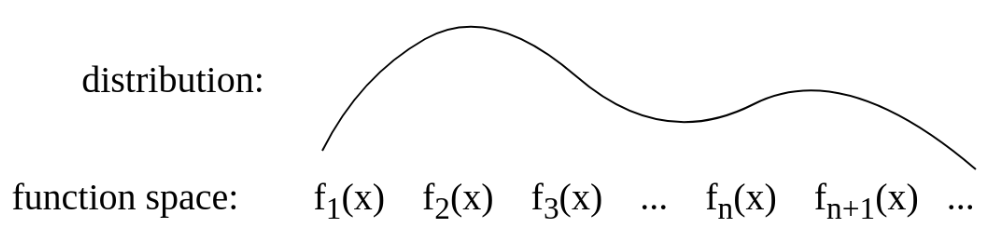
\includegraphics[width=0.9\linewidth]{Images/GP.png}
	\caption{Gaussian Processes are probabilistic models that define a distribution over functions.}
	\label{fig:gp}
\end{figure}
Many supervised learning problems can be seen as function approximations since a dataset of observations $ \{x_i, y_i\}^{n-1}_{i=0}$ is basically a number $n$ of evaluations $y_i = f(x_i)$ of an unknown function $f$. A supervised learning algorithm returns an approximated function $g$. The goal is to minimize the loss between the real function $f$ and the predicted one $g$. The evaluation is carried out on unlabelled data points $x_j$.

On the other hand, the disadvantages of Gaussian Processes are prior selection and training time for large datasets. Scaling issues with GPs have been addressed in \cite{snelson2006sparse}. The limited expressivity from functional restriction was addressed with DeepGPs in \cite{damianou2013deep}  \cite{salimbeni2017doubly}. Overcoming these issues and attempting to combine Deep Learning (DL) with GPs was proposed in \cite{wilson2016deep}, but the approach remains close to GPs since the network is used to learn more expressive kernels to use with GPs.

%%%%%%% CNP %%%%%%%
\section{Conditional Neural Processes}
In \cite{DBLP:journals/corr/abs-1807-01613}, the authors propose a novel research in which the inference potential of Gaussian Processes and the performance of neural networks are blended together. Neural networks are extensively employed as approximators of functions and have demonstrated considerable efficacy but often require large datasets for training. In CNPs, the prior knowledge is directly derived from the data, allowing them to infer the underlying function distribution based on observations. CNPs are built with three main blocks: Encoder, Aggregator, and Decoder. Encoder $E$ and Decoder $Q$ are typically Multi-layer perceptrons. The model structure is shown in Figure \ref{fig:cnp}. 
\begin{figure}
	\centering
	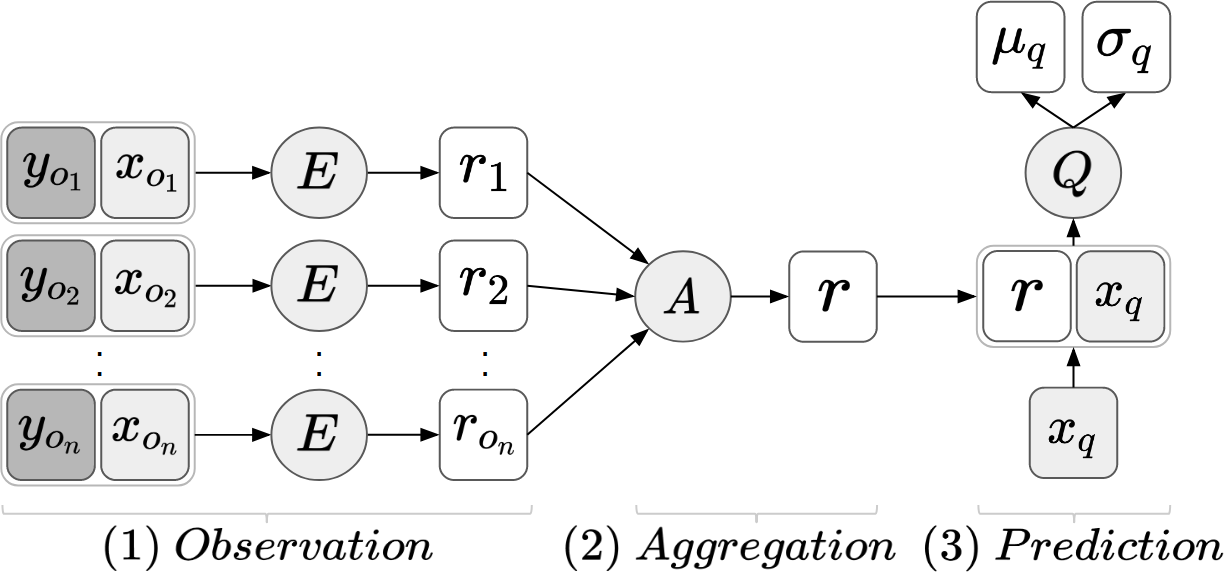
\includegraphics[width=0.5\linewidth]{Images/CNP.png}
	\caption{The structure of a CNP network, with three main blocks: Encoder, Aggregator, and Decoder.}
	\label{fig:cnp}
\end{figure}
The model scales with complexity $O(n+m)$ for making $m$ predictions from $n$ observations, while GPs scale with $O(n+m)^3$. CNPs don't require the specification of a kernel cause they learn it from the data provided in training. The tradeoff is that the representations of the observations have fixed dimensionality.

The work is based on the previous research of Neural Processes (NPs) \cite{garnelo2018neural}. NPs are suggested as a means to manage the substantial computational demands of GPs while leveraging their flexibility and efficiency with data. NPs help create different predictions by learning a shared hidden representation. However, they have trouble with long sequences because they automatically pick certain points. Building on NPs, Conditional Neural Processes (CNPs) are strong models that make training more efficient by allowing explicit conditioning.
\begin{figure}
	\centering
	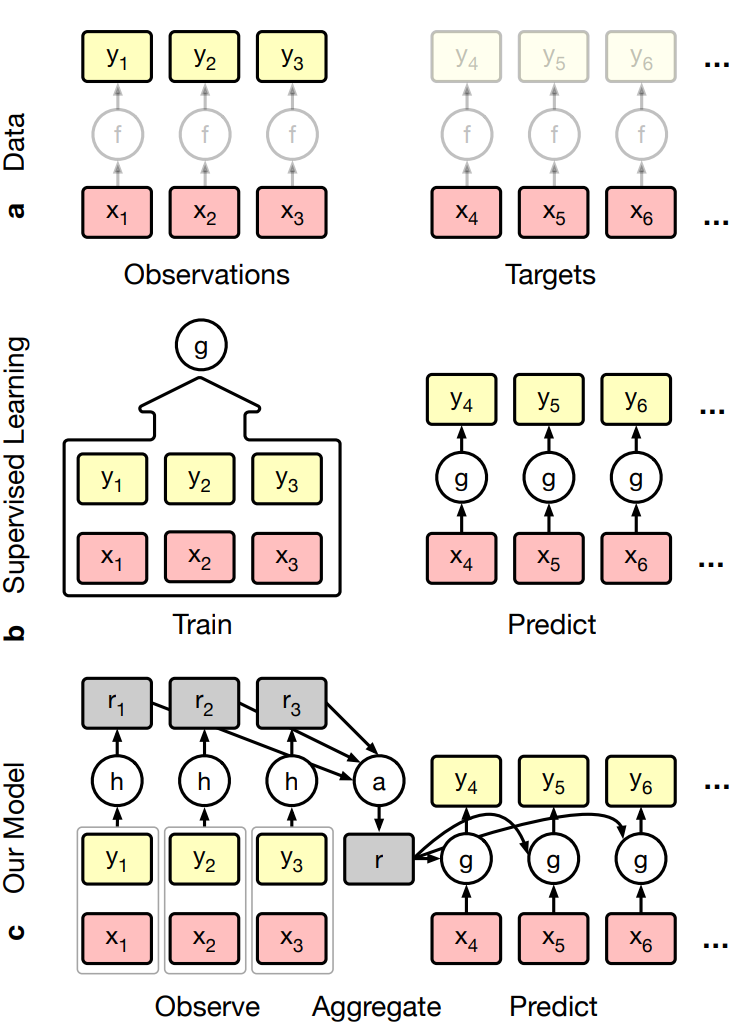
\includegraphics[width=0.5\linewidth]{Images/CNPdata.png}
	\caption{CNP allows precise predictions for targets sampled from a distribution conditioned with observations}
	\label{fig:cnp_data}
\end{figure}
The approach allows precise predictions for targets sampled from a distribution conditioned with observations, Figure \ref{fig:cnp_data}. Given a varying number of observations $O$, a neural network $E$ is utilized as an encoder to generate a fixed-size representation $r_i$.

Observations fed to the network don't have an order, following the stochastic processes, because subsequently, they are aggregated with the average operation to obtain a single representation $r$. Any commutative operation is valid and usable. The resulting representation $r$ contains the conditioning information and is fed to a decoder network $Q$ along with the desired target $x_j$ to query. The decoder network $Q$ has parameters $\theta$. For all the targets $x_j \in T$ the decoder outputs the mean and standard deviation.

The formulation of the encoding of each observation is:
\begin{equation}
r_i = E_\phi(x_i,y_i), \quad \forall(x_i,y_i) \in O
\end{equation}
and the following commutative operation between the encodings to create a single one: 
\begin{equation}
    r = r_1 \oplus r_2 \oplus ... \oplus r_i,
\end{equation}
The commutative operation expressed by $\oplus$, can be summation, average, product, and so on. 

The vector generated is concatenated with the target variables. The merged representation is passed to the decoder to obtain the output as:
\begin{equation}
    \phi_j = Q_\theta(x_j, r), \quad \forall x_j \in T
\end{equation}
Where the output is: 
\begin{equation}
    \phi_j = (\mu_j, \sigma_j^2)
\end{equation}
which are the mean and the standard deviation of the output variable.

In summary, the CNP model, with averaging operation, can be formulated as: 
\begin{equation}
    \mu_j, \sigma_j^2 = Q_\theta \left( x_j \oplus \frac{ \sum_{i}^{n} E\phi((x_i,y_i)) }{n}  \right)
\end{equation}

%%%%%%% CNMP %%%%%%%
\section{Conditional Neural Movement Primitives}
Finally, in \cite{Ugur-RSS-19}, Conditional Neural Movement Primitives are proposed as a model. CNMPs, as the name suggests, are an extension of CNPs and are particularly well suited for the robotics domain. The model illustration can be seen in Figure \ref{fig:cnmp}.  
\begin{figure}
	\centering
	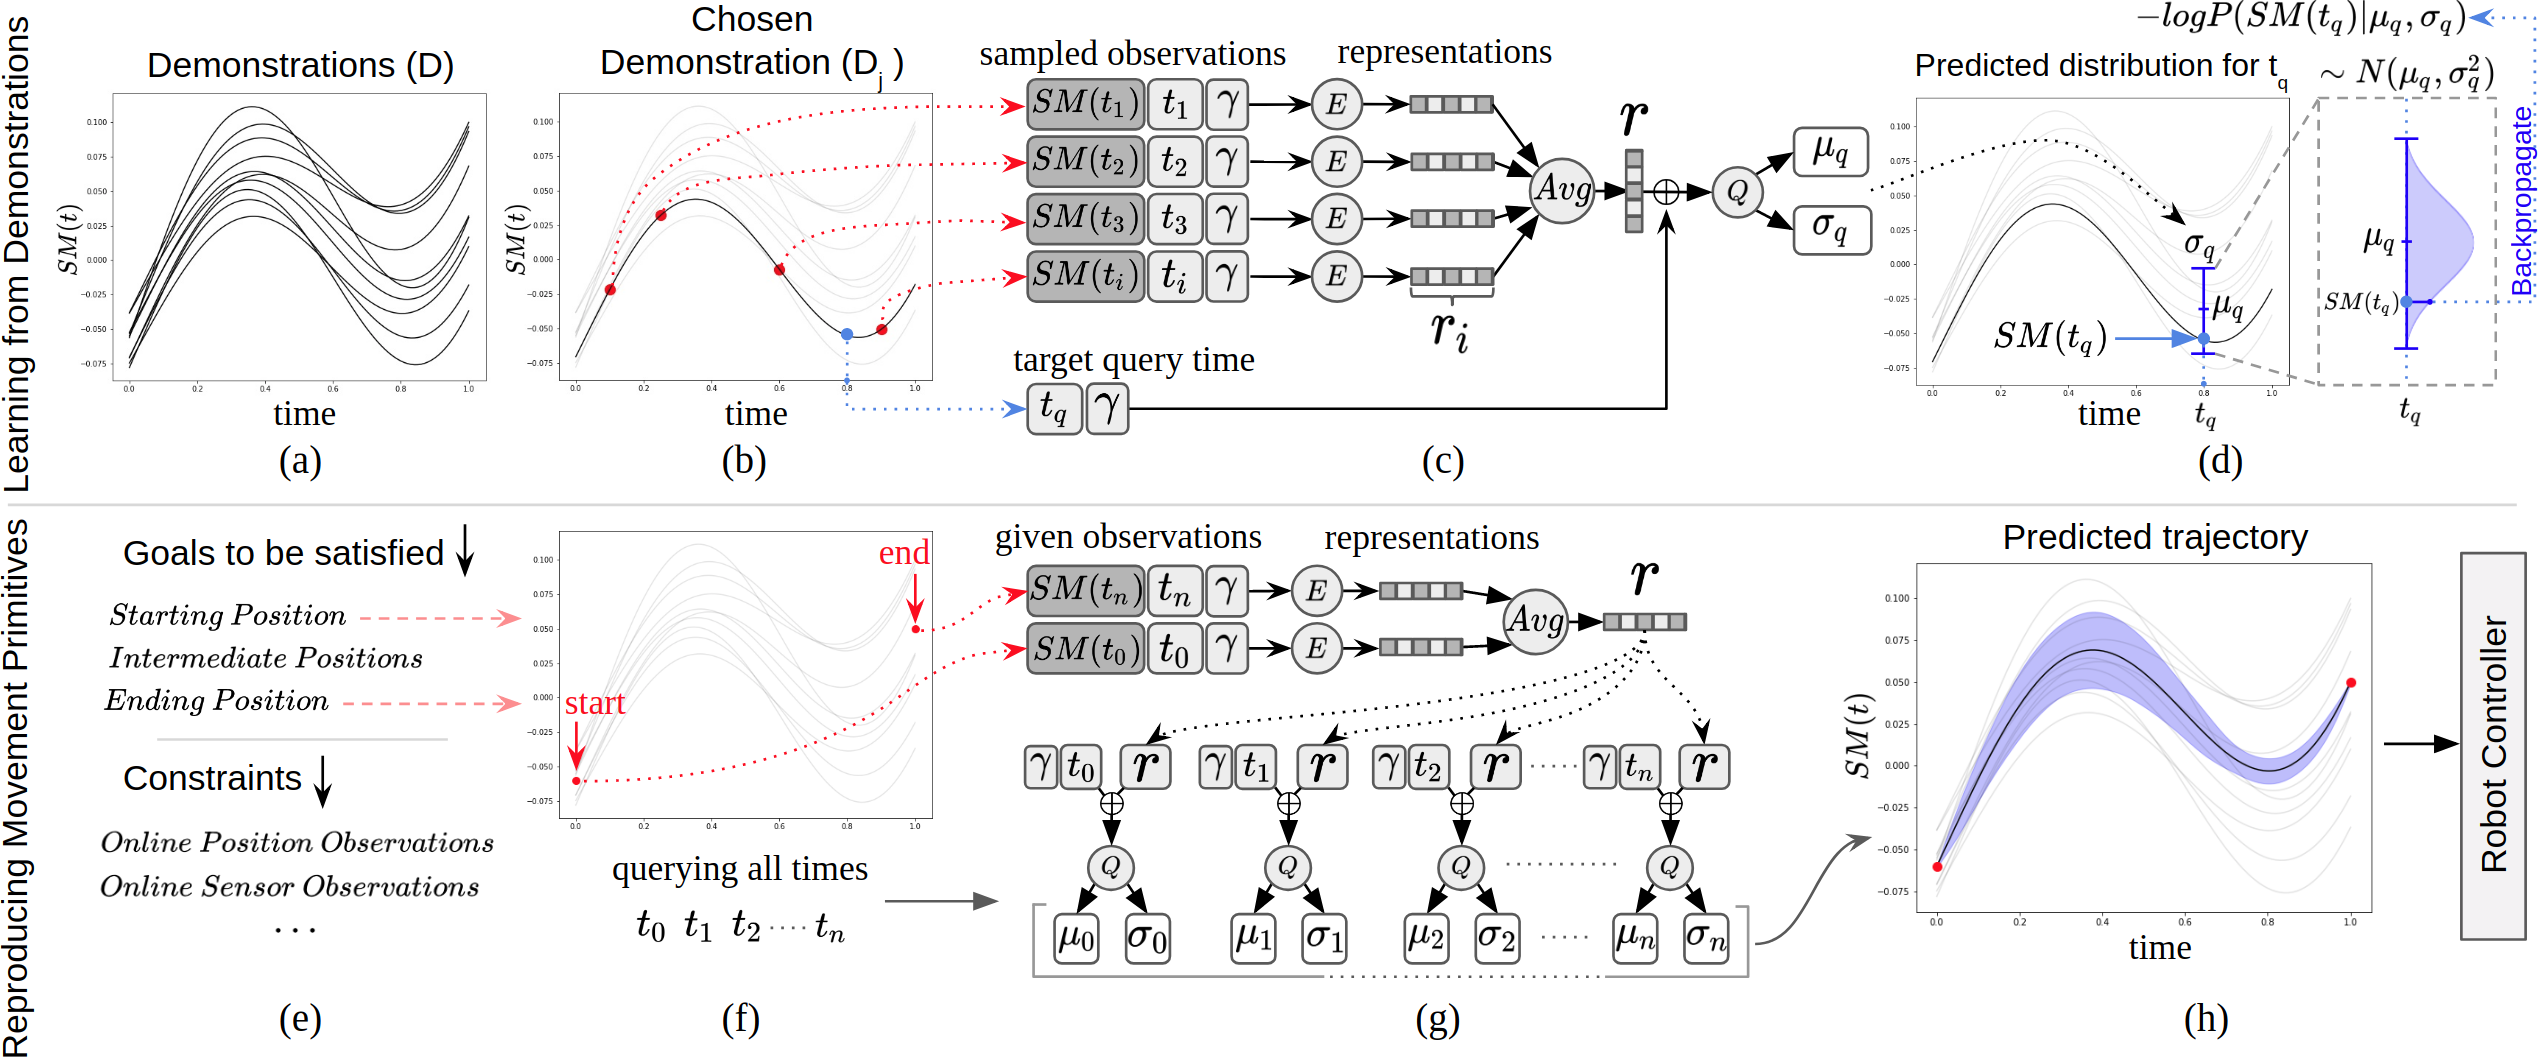
\includegraphics[width=0.9\linewidth]{Images/CNMP.png}
	\caption{CNMP model, it is conceived to work with temporal relations between sensorimotor data and different task parameters}
	\label{fig:cnmp}
\end{figure}
The "learning from demonstration" framework can learn non-linear relationships between trajectories and reproduce them in joint or task space. In this case, a trajectory is formally defined as a temporal function, $\tau = \tau (t)$, where the sensorimotor data in time describes how a robot moves. So, each trajectory $\tau$ is a list of ordered sensorimotor values: 
\begin{equation}
    \tau = \{ SM(t_1), SM(t_2), ... , SM(t_T ) \}
\end{equation}
where $SM(t_i)$ is the sensorimotor data at an instant of time $t_i$.
So, the challenge of trajectory generation becomes figuring out a series of commands $SM(t_i)$ that creates the movement desired \cite{gasparetto2007new}. 
Finally, with a set of observations $O$, the model has to learn the function $\tau = f(t|O)$, using $N$ expert demonstrations, $D = \{\tau_1, \tau_2, ... , \tau_N \}$. 

CNMPs are conceived to work with temporal relations $t$ and different task parameters $\gamma$. CNMPs maintain the permutation invariance of CNPs over observations $O$ and queries $T$. Furthermore, to make the model time-invariant, the sensorimotor trajectories are often scaled in the interval [0,1]. 
The task parameter $\gamma$ effectively adds one or more dimensionalities to the network's input, and it's passed to both the encoder and the decoder. An observation becomes the concatenation of $SM(t_i)$, $t_i$, and $\gamma$. The dimensionality of $SM(t_i)$ depends on factors like the Degrees of Freedom of the robot joints and the number of variables corresponding to the actuators. 
For the aggregation of the representations, the averaging operation has been chosen.
During training, a random trajectory $\tau_i$ is selected from the $D$ set of expert demonstrations. Next, a random number $n$ of random observation points are selected from the trajectory $\tau_i$. The encoder takes the $n$ observations and produces $n$ representations. The final representation is obtained by averaging the representations produced by the encoder fed with all the observation points. 
The target data is predicted using the representation and the query time $t$ concatenated to the task parameter $\gamma$

The encoder and the decoder are trained jointly with the error calculated from the following loss function:
\begin{equation}
    L(\theta, \delta)= -logP(y_i|\mu_i, softmax(\sigma_j))
\end{equation}
using both mean and standard deviation produced by the network.
As a note, the uncertainty of the prediction provided by the variance is useful for the model's active exploration to choose wisely where the next observations are needed.
Moreover, the capacity of CNMPs to deal with high-dimensionality input can also be used to input images in the model. Image completion indeed can be seen as a regression task.
Leveraging the interpolation capabilities of CNMPs, our approach will investigate novel synthesis by combining and concatenating previously taught ones.